
\documentclass{sig-alternate}
\usepackage[normalem]{ulem}
\usepackage[usenames,dvipsnames]{pstricks}

\usepackage{mathtools}

\usepackage{algorithm2e}

\usepackage{ctable}
\usepackage{url}
\usepackage{multirow}

\begin{document}
\conferenceinfo{WSDM}{'14 New York City, NY, USA}
\title{Efficient Temporal Synopsis of Social Media Streams}

\maketitle
\begin{abstract}


%Search and summarization of 
Mining
streaming social media, such as Twitter, requires the ongoing analysis of large volumes of data with dynamically changing characteristics.  Tweets are short and repetitious~--~lacking context and structure~--~making it difficult to generate a coherent synopsis of events within a given time period.  Although some established algorithms for frequent itemset analysis might provide an efficient foundation for synopsis generation, the unmodified application of standard methods produces a complex mass of rules, dominated by common language constructs and many trivial variations on topically related results.  Moreover, these results are not necessarily specific to events within the time period of interest.  To address these problems, we build upon the Linear time Closed itemset Mining (LCM) algorithm, which is particularly suited to the large and sparse vocabulary of tweets.  LCM generates only closed itemsets, providing an immediate reduction in the number of trivial results.  To reduce the impact of function words and common language constructs, we apply a filtering step that preserves these terms only when they may form part of a relevant collocation.  To further reduce trivial results, we propose a novel strengthening of the closure condition of LCM to retain only those results that exceed a threshold of distinctiveness.  
We also propose a clustering scheme that removes redundancy from
the mining results.
%Finally, we perform temporal ranking, based on information gain, to identify results that are particularly relevant to the time period of interest.  
We evaluate our work over a collection of tweets gathered in late 2012, exploring the efficiency and filtering characteristic of each processing step, both individually and collectively.  
%Based on our experience,
By performing temporal ranking, based on information gain, we identify results that are particularly relevant to the time period of interest.
Based on our experience, the resulting synopses from various time periods provide understandable and meaningful pictures of events within those periods, with potential application to tasks such as temporal summarization and query expansion for search.
\end{abstract}
%\category{H.4}{Information Systems Applications}{Miscellaneous}
%A category including the fourth, optional field follows...
%\category{D.2.8}{Software Engineering}{Metrics}[complexity measures, performance measures]

%\terms{Theory}

%\keywords{ACM proceedings, \LaTeX, text tagging}
\newpage
\section{Introduction}

Mining social media text poses unique challenges
because of the text's content and form.
The user generated content includes a substantial 
amount of social chatter, 
which ought to be filtered out by mining algorithms.
In terms of form, social media posts are short thus
undermining the effectiveness of within document 
term frequency counting.
They also lack structure and other formatting cues,
thus important terms cannot be pinpointed easily. 
Moreover, the rate at which users generate and consume
social media posts necessitates the use of efficient algorithms
to provide users by real-time mining results.
To realize the benefits of social media in giving a voice to ordinary people,
it is desirable to devise techniques that focuses on the content of posts.

In this work we study the use of frequent itemset mining
to create a synopsis of social media streams. 
Frequent itemset mining is suitable to the dynamic nature of social media streams.
It does not require prior knowledge of the distribution of items,
nor does it require selecting a few items to monitor 
or a number of topics to mine. 
It is fast, efficient and scalable.
However, frequent itemset mining is not readily suited for application on text
without preprocessing steps that are difficult to apply to social media text;
for example, stop word removal which requires language identification
to be done before it, and will thus suffer from the poor performance
of language identification on social media~\cite{bergsma2012language}.
In our experience, directly applying frequent itemset mining algorithms
to social media text results in myriads of itemsets that are 
mostly meaningless, repetitive or bear no information.
In this work we address the shortcomings of 
frequent itemset mining which lead to such poor performance.
As a result, the frequent itemset mining results become
suitable for use as a synopsis representing what is happening
on social media at different points of time. 
The synopsis is particularly rich because it
includes the itemsets as well as the ids of posts in which they occur.

Frequent itemset mining was originally proposed as a preliminary stage for
association rules mining.
It produces a large number of itemsets, which
has to be further processed to 
produce a smaller number of association rules.
Furthermore, the number of itemsets grows with the number of
distinct items, which is particularly high in the text domain.
To reduce the number of itemsets, they may be limited by setting a high
frequency threshold, but this is not possible in text mining because
frequencies of items follow a long-tailed Zipfean distribution.
We propose a condition for selecting informative itemsets, 
and a clustering scheme for reducing redundancy in the mining results.
Our methods exploit the dynamics of social media 
and make use of the collaborative filtering
that users naturally undergo on social media, 
by sharing interesting posts and participating in conversations.


We process the social media stream in batches 
of data from consecutive epochs of time.
We propose a formula for ranking the itemsets
in the synopsis of each epoch according to temporal novelty.
An empirical evaluation of the effectiveness of our proposed methods
shows that the hour by hour synopses at different times 
actually reflects what was happening at those times. 
It is easy to see that
we achieve improvements over a baseline
of applying unmodified frequent itemsets mining, 
in terms of the reduction in the number of itemsets 
and the quality of individual itemsets.
We also make an effort to compare our synopses 
with those generated by a state of the art algorithm 
for summarization based on itemset mining, MTV~\cite{mampaey2011tell}.
However, the number of topically relevant itemsets our algorithm mines 
is much larger than what MTV can mine in reasonable time,
inhibiting the use of standard comparison measures.
The large number of topics in the mining results 
also impede the use of quality measures which require 
the creation of a gold standard, 
such as those proposed for evaluating
key-phrase extraction algorithms~\cite{Zhao:2011:TKE:2002472.2002521}.

For the purpose of evaluation, we show the synopses 
of periods of time when it is known what 
social media users are expected to be talking about.
Specifically, the day of the U.S. presidential elections,
and periods in which Google Top Charts\footnote{\scriptsize \texttt{http://www.google.ca/trends/topcharts\#vm=chart\&cid=people\&\\geo=US\&date=201211}}
show high volume of queries about certain celebrities.
The synopses of all hours in the last 3 months of 2012
are available for download\footnote{\scriptsize \url{http://blinded.blinded.com/blinded/thesis_results/twitter_synopses/1hr+30min_ngram5-relsupp10_oct-nov-dec/}}. 
%http://plg.uwaterloo.ca/~yaboulna/


As a merit of using frequent itemset mining, the synopses include
itemsets about topics with sustained user interest as well as a spike of interest
--~unlike trending topics\footnote{\scriptsize \url{http://blog.twitter.com/2010/12/to-trend-or-not-to-trend.html}}
\cite{mathioudakis2010twittermonitor} which are limited to
topics showing spikes of interest.
The mined itemsets provide the vocabulary associated with events and can be
used as a preliminary step for search and summarization.
For example, the collection of mining results from different epochs of time
can be used for temporal query and document
expansion~\cite{choi2012temporal, efron2012improving}. 
The results from each epoch can be treated as a document, facilitating the
creation of a ``temporal profile''~\cite{jones2007temporal} of the query
or a document being expanded.
For summarization, frequent itemsets can provide a good foundation for summary
creation.
While the frequent itemsets themselves are not summaries, since they lack
qualitative properties such as coherence and cohesion, the results are
understandable at the user level.

The rest of the paper is organized as follows.
The next three sections provide necessary background.
We start by discussing related work in section \ref{sec:related},
we then explain frequent itemset mining and the algorithm on which we build
our work in sections \ref{sec:fim} and \ref{sec:lcm} respectively.
In sections \ref{sec:socmine} and \ref{sec:strong} we
propose solutions to the problems faced when applying frequent
itemset mining to social media text. 
Section \ref{sec:socmine} deals with the large number of language
constructs and reduces the number of itemsets.
In section  \ref{sec:strong} we propose a condition for selecting
itemsets and filtering out ones that are not \emph{distinct} from 
their subsets, and we propose a clustering that merges
together similar itemsets into \emph{strongly closed itemsets}.
In section \ref{sec:rank} we introduce a ranking formula
specially tailored for ranking \emph{strongly closed itemsets}.
We use this formula to rank itemsets and construct 
the examples used for evaluation. 
Finally, section \ref{sec:concfut} concludes our presentation and
suggests future directions.


\section{Related Work}
\label{sec:related}
Frequent itemset mining comprises a large body of work that goes back to the
early 1990s.
We cover the topic only briefly, as the focus of this paper is not frequent
itemset mining but rather its adaptation to social media text.
The original Apriori algorithm~\cite{agrawal1994fast} and algorithms based on
it suffer performance degradation and  large increases in memory requirement
when the number of distinct items is high.
These limitations are caused by a candidate generation bottleneck,
as explained later.
Another well-known class of mining algorithms are the
FP-Growth~\cite{han2000mining} based algorithms.
FP-Growth skips the candidate generation step, and instead creates a succinct
representation of the data as a frequency ordered prefix tree called the
FP-tree.
An FP-tree imposes the invariant that within each branch the frequency is
non-increasing from the root down to the leaves. 
The memory requirements of the FP-Growth algorithm suffers from the sparsity
of data, since the data structure is succinct only if it can find common
prefixes within the constraints of its invariant. 
Another algorithm, not as widely used but robust against data sparsity, is
Linear-time Closed itemset Mining (LCM)~\cite{uno2004lcm},
which we will describe in detail in section \ref{sec:lcm}.
As a starting point for our work, we use the implementation of LCM submitted
to the workshop for Frequent Itemset Mining Implementations (FIMI) in
2004~\cite{DBLP:conf/fimi/2004}, which was the workshop's award winner. 

The problem of having many itemsets, with redundancy and noise, can be addressed by
picking out  representative itemsets that satisfy a certain condition
that reduces redundancy in the mining results (itemsets and their support information).
The closure condition~\cite{pasquier1999discovering} is a prominent condition
upon which many other conditions are based.
Most similar to the \emph{distinct} itemsets we propose in this paper
are the $\delta$-covered~\cite{xin2005mining} and the
$\delta$-free~\cite{boulicaut2003free} sets.
The $\delta$-covered condition is exactly the opposite of the \emph{distinct}
condition, and it ``relaxes the closure condition to further reduce pattern
set size'' \cite{liu2012finding}.
The $\delta$-free condition is similar to the \emph{distinct} condition,
but it is used to eliminate different itemsets, since its motivation
is to provide a compressed representation of itemsets by sacrificing support
information. 

Another approach to picking out itemsets is choosing ones that 
can be used to compress the data. The KRIMP algorithm~\cite{vreeken2011krimp} is 
a good example of methods that follow this approach. Our goal is different because
we aim to filter out itemsets pertaining to personal updates, which make up a large
portion of social media data. 
A similar goal is sought by the Maximally informaTiVe itemsets (MTV) algorithm~\cite{mampaey2011tell}. 
MTV uses a maximum entropy model to judge if an itemset is redundant, finally choosing the
top K itemsets according to the KL-Diverge between the itemset's  frequency and  the model's estimate. 
In this work we focus on efficiency, allowing the summary to include larger numbers
of itemsets than the values of K for which MTV is efficient.
This is crucial for scalability to the volumes of data typical of social media streams.
However, we compare our results to the ones obtained from MTV.

Likewise, Yan et al.~\cite{yan2005summarizing} choose 
K \emph{master} patterns as representatives of the data. 
A \emph{master} pattern is the union of all itemsets in a 
cluster, similar to our proposed \emph{strongly closed itemset}. 
While the use of clustering is similarly motivated by 
the trivial difference between itemsets, 
the K \emph{master} itemsets  have to cover the whole data, 
unlike the \emph{strongly closed itemsets} which actually 
avoid clustering together different topics or different opinions within a topic.

Our work complements the work done by Yang et al.~\cite{yang2012framework} for using 
frequent itemsets to build a temporal index on social media posts. 
They use frequent itemsets to decrease the space requirements of the index,  
but they choose itemsets to include in the index based on their utility in compressing the data. 
We propose methods to choose itemsets that are topically relevant, 
making use of the nature of social media.


The use of frequent itemsets for improving search performance has been considered before. 
For example, in Li et al.~\cite{li2010mining} itemsets are mined from
paragraphs of newswire text, and are used to determine term weights for query
expansion.
Improvements in performance have been achieved by using itemsets taken from
a training set of related documents, as well as ones from unrelated documents.
Related methods for term weighting were
used in pseudo-relevance feedback for Twitter search~\cite{abounlaga2012frequent,laumicroblog},
and achieved substantial improvements over a baseline.
Our work can provide such methods by a short ranked list of itemsets.

Existing techniques for summarization and topic extraction were adapted for social media.
Zhao et al.~\cite{Zhao:2011:TKE:2002472.2002521} build summaries based on 
an adaptation of Latent Dirichlet Allocation (LDA) for Twitter.
Parikh and Karlapalem~\cite{parikh2013events} extract topics 
from Tweets using a simplified state machine for burst detection.
The short length of social media text is overcome by 
applying the adapted techniques on large batches of posts made in a long period of time. 
Our method processes data in batches as small as an hour worth of posts, 
resulting in temporally relevant synopses. 
Petrovi\'{c} et al.~\cite{petrovic2010streaming}
used an adaptation of Locality Sensitive Hashing (LSH) %~\cite{indyk1998approximate} 
to perform first story detection at scale.
Their system clusters tweets efficiently,
but it does not achieve high precision in 
determining if a tweet cluster
pertains to an event or not.

The use of Twitter to provide a summary of a specific event 
has also been studied. 
Chakrabarti and Punera~\cite{chakrabarti2011event} track 
tokens appearing in tweets tagged by the name of an American football team,
and use them to create a summary of a game using statistically improbable phrases.
Sharifi et al.~\cite{sharifi2010summarizing} also use phrases from tweets about a user specified event.
Their method ends up to be very similar to frequent itemset mining,
but uses a graph of terms.

\section{Frequent itemset mining}
\label{sec:fim}
\subsection{Preliminaries}
Classically, frequent itemset mining is applied to a \emph{database} of
\emph{transactions} made at a retail store.
This terminology is suitable for market basket data and we retain it out of
convention, even though we are mining text where the terms ``corpus'' and
``document'' are normally used.
Because of the dynamic nature of social media, rather than giving the whole
database as input to mining algorithms, the input is an \emph{epoch} of data;
data with timestamps within a certain period of time.
The epoch's \emph{span} is the length of this period in hours,
and the \emph{volume velocity} at this epoch is the number of transactions in the epoch
divided by its \emph{span}.

A \emph{frequent itemset} is a set of items that occur together a number of
times higher than a given threshold, called the \emph{support} threshold.
We adapt the support threshold to the dynamicity of the \emph{volume velocity} at
different times of the day.
We define the \emph{minimum support threshold} as the threshold at the hour
of the least \emph{volume velocity} during the day.
The \emph{minimum support} is supplied as an absolute number, $a$, and then
converted to a ratio, $\alpha = \frac{a}{\textbf{avg}(\min_{day}{(vol.\, vel.)})}$.
The actual support threshold used for mining any given epoch is thus
$\alpha$ multiplied by the number of transactions. 
We now introduce the notation used in this paper:
\begin{itemize}
\item $W = \{w_1,w_2,\ldots, w_n\}$: The set of all items appearing in an \emph{epoch}. 
We use term N-grams in this paper.
\item $t_a = \{w_{a1},\ldots, w_{am}\}$: A transaction made up of a set of items. Each transaction has a sequential id, denoted by the subscript letter, derived from its timestamp.
\item $E^{span} = \langle t_a, t_b, \ldots, t_v\rangle$: An epoch of data of a certain span, such as an hour, made up of the sequence of the transactions created within this hour.
\item $s \subset W$: An itemset; any possible combination of items. 
\item $T_s = \{t: t \in E \, and \, s \subseteq t\}$: All transactions containing itemset s. We refer to it as the itemset's postings list.
\end{itemize}

\subsection{Fundamentals}

The two basic operations of frequent itemset mining algorithms are
\emph{candidate generation} and \emph{solution pruning}.
The original Apriori algorithm by Agrawal et al. \cite{agrawal1994fast}
generates candidates of length K (K-itemsets) by merging frequent itemsets of
length (K-1) ((K-1)-itemsets) that differ in only 1 item, usually the last
item given a certain total ordering of items.
By using only the frequent  (K-1)-itemsets for generating candidate K-itemsets,
many possible K-itemsets are implicitly pruned, based on the downward-closure property:
all subsets of a frequent itemset must be frequent.
This approach still can generate a large number of candidates, especially
in early iterations of the algorithm.
Consider, for example, the generation of candidate 2-itemsets from a database.
This generation requires producing all unordered pairs of 1-itemsets (terms),
after pruning out rare ones with frequency less than the support threshold.
In many domains, including text mining, the number of frequent 1-itemsets is
large enough to prohibit generating a number of candidates in the order of this
number squared.
In text mining, a rather low support threshold has to be used, because the
frequency of terms follow a long-tailed Zipfean distribution.

\section{Basic Algorithm}
\label{sec:lcm}
To overcome the bottleneck of \emph{candidate generation}, many proposed
algorithms take hints from the transaction space rather than operating blindly
in the item space.
Some of these algorithms operate by traversing a data structure representing
the transactions~\cite{han2000mining}; others generate itemsets having
specific properties that help in pruning out more candidates.
In this paper, we expand on LCM \cite{uno2004lcm}, an algorithm based on a
property of a class of itemsets called
\emph{closed itemsets}~\cite{pasquier1999discovering}.
A closed itemset contains any item that is present in all the transactions
containing this itemset.
A formal definition of closed itemsets is given in equation \ref{eq:Closed}: 

\begin{equation}\label{eq:Closed}\mathcal{C} = \{s_c:\, s_c \subset W \, and \,\nexists \, s_d \, where \, s_c  \subset s_d \, and \, |T_{s_c}| = |T_{s_d}|\}\end{equation}

The properties of closed itemsets are as follows:
\begin{enumerate}
\item Adding an item to a closed itemset reduces its support. 
\item A subset of a closed itemset is not necessarily closed, but one or more closed subset must exist for any itemset (formally this could be the empty set, given that any item that appears in all transactions is removed in a preprocessing step). 
\item If a closed K-itemset can be extended any further then one of its supersets will be closed, however not necessarily a (K+1) superset. Itemsets that cannot be extended any further are called \emph{maximal itemsets}, which form a subclass of closed itemsets.
\end{enumerate}

Besides being much smaller than the solution space of frequent itemsets,
the solution space of closed itemsets can be navigated efficiently.
By using an arbitrary total ordering of items, any closed itemset can be
considered an extension of exactly one of its subsets.
Thus, only this subset is extended during candidate generation.
All other subsets do not need to be extended by items that would lead to
the longer closed itemset.
This property is called \emph{prefix preserving closure extension
(PPC-Extension)} and it was proposed and formally proved by
Uno et al.~\cite{uno2004lcm}.
\emph{PPC-Extension} is achieved by following three rules, which we state
after a few definitions to facilitate their statement.
First, an item is \emph{larger/smaller} than another item if it comes
later/earlier in the total ordering.
This terminology comes from the fact that LCM is most efficient if the items
are ordered in ascending order of their frequency.
Second, the \emph{suffix} of an itemset is one or more items 
which have to be removed to get
an itemset with greater support.
Notice that they will necessarily be at the end of the itemset,
regardless of the total ordering.
Finally, we call the first item added to the suffix of the itemset its
\emph{suffix head}.
With this terminology, the rules for \emph{PPC-Extentsion} are:
\begin{enumerate}
\item An itemset must be extended by every item that occurs in $T_{itemset}$, 
except items which are \emph{smaller} than its \emph{suffix head};
extending by \emph{smaller} items will lead to closed itemsets already generated in an earlier step. 
\item After adding an extension item, $w_e$, to an itemset, $s$, we add all other items that appear in all transaction containing $s \cup \{w_e\}$.
The added items are the \emph{suffix}.
\item If all items in the \emph{suffix} are \emph{larger} than the \emph{suffix head} then add the itemset to the solution. Otherwise, prune this solution branch; all closed itemsets within this branch have already been generated. 
\end{enumerate}
 
Table \ref{table:PPCExample} is an example of how \emph{PPC-Extentsion} is
used to generate closed itemsets starting from the
\emph{1}-itemset \{`barack'\}.
The upper table enumerates $T_{\{`barack'\}}$.
The lower table shows steps of itemsets generation.
The current itemset along with its frequency is in column 2.
Itemsets marked by an (*) are the closed itemsets that are part of the solution.
The suffix of the itemset is shown in \emph{italic}. 
All possible extension items and their frequencies are in column 3. 
Extension items that are \emph{smaller} than the \emph{suffix head} 
are shown with a line striked through them. 
For each itemset, the extension items are kept 
so that it is known which extension item 
is next in turn to be added.
An item is bolded when its turn to be added has come.
After adding each item, a pass is done on $T_{itemset}$ to 
enumerate and count possible extension items.
To enforce a support threshold, infrequent extension items would be removed
after counting, 
but in this example there is no such threshold.
Finally, column 4 is a comment explaining each step.


Table \ref{table:PPCExample} shows that the number of steps is linear in the number of closed itemsets,
and the only additional storage required, besides storage for the documents,
is that required for possible extension items.
Of course, this is a simplified example, but it shows in essence how LCM
achieves its low run time and memory requirements.
We refer the interested reader to Uno et al.~\cite{uno2004lcm} for a
theoretical proof that the algorithm runs in linear time in the number of
closed itemsets,
and that this number is quadratic in the number of transactions.
Performance on a real dataset is shown in section \ref{sec:socmine}.
We proceed by describing how to implement this algorithm. 


\begin{table*}

\centering
\begin{tabular}{|c|p{6cm}||c|p{6cm}|} \hline
\textbf{Doc. Id} & \textbf{Document} & \textbf{Doc. Id} & \textbf{Document}\\\hline
a& barack \& mitt & b & barack obama \& mitt romney  \\\hline
c& barack obama \& romney & d & barack obama  \\\hline
\end{tabular}
\begin{tabular}{c}
Documents (two per row)\\\\
\end{tabular}

\begin{tabular}{|c|p{5cm}|p{5cm}|p{5.5cm}|} 
\hline
\textbf{Step}&\textbf{Current Itemset}&\textbf{Possible Extension Items}&\textbf{Comments}\\ \hline

1& \{barack\} (4) & mitt (2), obama (3), romney (2) & {\small Items in $T_{\{`barack'\}}$ are counted. }\\\hline 
2& \{\emph{barack}\} (4)* & mitt (2), obama (3), romney (2) &  {\small Rule 3: suffix is ordered, emit itemset.  } \\ \hline
3& \{\emph{barack}\} (4) & \textbf{mitt} (2), obama (3), romney (2) &  {\small Items are ordered lexicographically.} \\ \hline
4& \{barack, \emph{mitt}\} (2)* & \textbf{obama} (1), romney (1) &  {\small Extension items reenumerated \& counted.}\\\hline
5 & \{barack, \emph{mitt}, obama\} (1) & romney (1)                       &  {\small Rule 2: `romney' appears in all $T_{itemset}$. } \\\hline
6 & \{barack, mitt, \emph{obama, romney}\}(1)* & & {\small Rule 3: `obama'  is the \emph{suffex head}. } \\\hline
7 & \{\emph{barack}\} (4) & mitt (2), \textbf{obama} (3), romney (2) &  {\small Nothing more to add, back to \{`barack'\}.}\\\hline
8 & \{barack, \emph{obama}\} (3)* & \sout{mitt} (1), \textbf{romney} (2) &  {\small Rule 1: skipping `mitt', adding `romney'  } \\\hline
9 & \{barack, obama, \emph{romney}\} (2)* & \sout{mitt} (1) &  {\small Rule 1: Nothing more to add.  } \\\hline
10 & \{\emph{barack}\} (4) & mitt (2), obama (3), \textbf{romney} (2) &  {\small Back to \{`barack'\}, adding `romney'. } \\\hline
11 & \{\emph{barack}, romney\} (2) &  mitt (1), obama (2) &  {\small Rule 2: add `obama' after `romney'. } \\\hline
12 & \{barack, \emph{romney, obama}\} (2) &  \sout{mitt} (1)  &  {\small Rule 3: suffix is not ordered, prune.} \\\hline
13 & \{\emph{barack}\} (4) & mitt (2), obama (3), romney (2) &  {\small All possible extension items were added. } \\\hline
\end{tabular}
\begin{tabular}{c}
Closed itemsets containing `barack'
\end{tabular}

\caption{Generation of closed itemsets by Prefix Preserving Closure Extension}
\label{table:PPCExample}
\end{table*}


\subsection{Implementation Details}
We show in algorithm~\ref{algo:lcmix} how to implement LCM and PPC-Extension
using an inverted index.
The inverted index is part of the standard text search infrastructure,
and it is also a  good representation of textual data. 
Other representations that are designed for databases in general
might not be well suited for such sparse data with a large number of items. 


The algorithm takes as input an epoch of data and a support threshold as a
ratio $\alpha$.
It outputs the closed itemsets with support above the threshold.
Along with each itemset in the solution, it also outputs the transactions
in which it occurs~--~which is represented as $\langle items,
T_{itemset} \rangle$.
The symbol $\succ$ denotes that the lefthand side  succeeds the righthand
side in the total ordering of terms. 

\begin{algorithm}
\SetAlgoLined
\LinesNumbered
\SetKwProg{Fn}{Function}{ is}{end}
\KwIn{$\alpha$: Dynamic support ratio}

\KwData{E: Epoch of data}
\KwResult{C: Closed itemsets having support $\alpha$ within E}
C $\gets \{\langle \emptyset, E\rangle\}$ \tcp*{$\emptyset$ is a closed itemset}
X $\gets$ Inverted index of E\;
\ForEach{$w \in X.tokens$}{
	$T_{\{w\}} \gets$ X.postingsList[$w$]\;
	\lIf{$|T_{\{w\}}| \geq \alpha \frac{|E|}{E.span}$}{
		LCM($\{w\}, w, T_{\{w\}}$)
	}
}
\Return{C}\;

\Fn{LCM(s: Current itemset,   $w_{sh}$: Suffix head, \\ $T_s$: Transactions (tweets) containing s)}{
	freq[$1 \ldots w_n$] $\gets$ 0\tcp*{Initialize freq. counts}
	suffix $\gets \{ w_{sh}\}$\;
	\ForEach{$t \in T_s$}{
		\ForEach{$w \in t$}{ 
			freq[$w$]++\;
			\lIf{freq[$w$] $ = |T_s|$}{
				suffix $\gets$ suffix $\cup\, \{w\}$
			}
		}
	}
	\lIf{$\exists v \in$ suffix: $w_{sh} \succ v$ }{
		\Return
	}
	C $ \gets $ C $ \cup\, \{\langle s \cup {suffix}, T_s\rangle\}$\;
	\ForEach{$v \succ w_{sh}$ and $v \notin $ suffix}{
		\If{freq[$v$] $\geq \alpha \times |E|$}{
			$T \gets T_s \cap v$	\tcp*{Results of query $s$ AND $v$}
			LCM($s \cup suffix \cup \{v\}, v, T$) 
		}
	}
}

\caption{LCM frequent itemsets mining}
\label{algo:lcmix}
\end{algorithm}

\section{Mining social media}
\label{sec:socmine}

Throughout this paper we use data collected from the Twitter public
stream\footnote{\scriptsize \url{https://dev.twitter.com/docs/streaming-apis/streams/public}}
since October 1st, 2012. 
We collect only tweets written in the Latin script to facilitate tokenization
using white space and other word boundaries.
%The average number of such tweets per hour is 119,035.49.
The average number of tweets collected per day is 2,779,091.82 tweets.
%without removing days with interruption: 2,705,931.83 tweets.
We collect only the tweet text to avoid reliance on any features specific to a
certain social medium,
and to make the algorithms applicable to other media where text is short  
% such as Facebook or Google+ status updates.
such as YouTube comments.
The only preprocessing we performed was to remove duplicate original tweets
(not retweets) using a Bloom filter.
This filtering removes spam tweets sent by botnets, averaging at 2.86\% of the stream. 
%3352.61069856614 / 116920.214769629

We apply the algorithms to epochs of data, so they are not strictly stream
processing algorithms.
However, we regard the process as mining a sliding window that is moved
forward by time steps of short span.
The time step must be longer than the time needed to mine an epoch of data,
and the performance of our algorithms makes it possible to use a time step
of a few seconds for epochs up to a day long.
Figure \ref{fig:runtimeEpochs} shows the runtime of LCM on epochs of
increasing length, and we will show in section \ref{sec:bounding} that our
extensions do not degrade performance.
The times reported in figure \ref{fig:runtimeEpochs} are averages across all
epochs of the specified length in the last 3 months of 2012, % October, November and December,
using a time step that is half the epoch length.
The \emph{minimum support} threshold we use throughout this paper
is 10 occurrences in the hour of least \emph{volume velocity},
which translates into $\alpha = 0.0002$.

In the rest of this paper we mine epochs of 1 hour span.
The reason behind this choice is our observation that the number of closed
itemsets mined from epochs of span 1 hour or more,
at the same support threshold, remains the same.
This indicates that itemsets mined from shorter epochs of social media text
are not included in the results of mining longer epochs. 
Therefore, the epoch span should be minimized.
However, when the epoch span is shorter than an hour the frequency required
to surpass the support threshold becomes very low,
and number of mined itemsets increases, with many noise itemsets appearing in
the results.

Regardless of the length of the epoch,
many mined itemsets are combinations of function words.
In the next section, we outline how we reduce the number of itemsets and
eliminate the effect of function words by N-gram filtering.

\begin{figure}
\centering
\scalebox{.4} 
{
\begin{pspicture}(0,-5.61)(19.94,5.61)
\rput(9.97,0.0){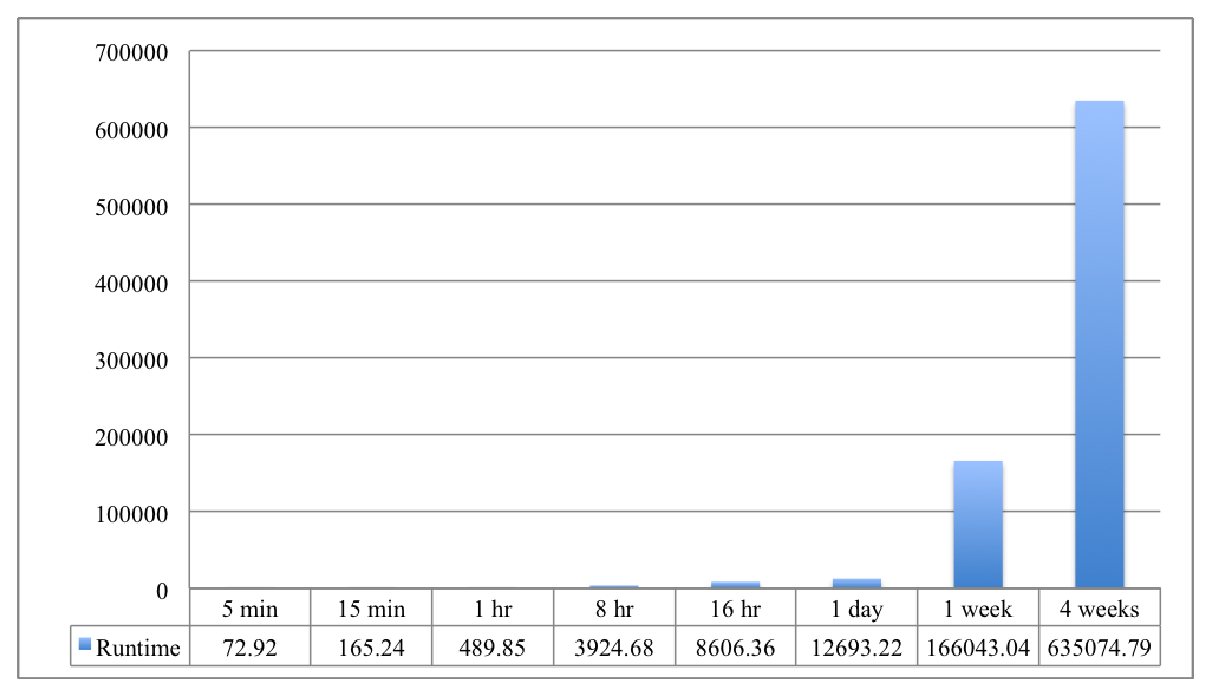
\includegraphics{runtime_different-epoch-spans_bar-table.eps}}
\rput(9.8,1.44){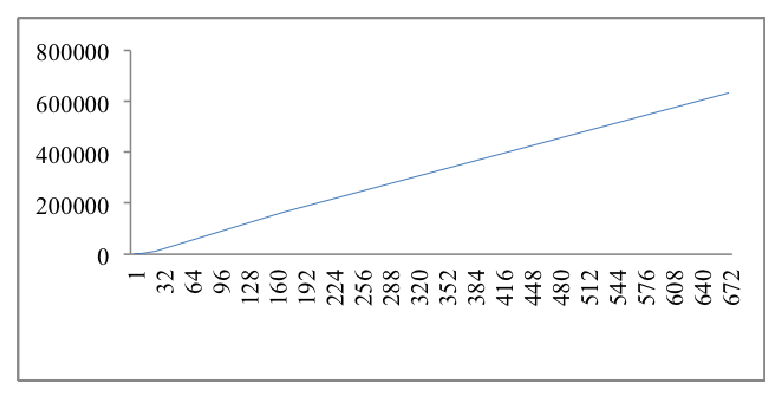
\includegraphics{runtime_different-epoch-spans_line.eps}}
\usefont{T1}{ptm}{m}{n}
\rput{90.15449}(0.96138316,-0.45039606){\rput(0.6871191,0.225){\LARGE Time in milliseconds}}
\usefont{T1}{ptm}{m}{n}
\rput(10.130039,-0.925){\Large Epoch span in hours}
\end{pspicture} 
}
\caption{Mean runtime at different epoch spans}
\label{fig:runtimeEpochs}
\end{figure}

\subsection{Mining Term N-grams}
\label{sec:ngrams}



\begin{figure*}[htb]
\centering
\scalebox{0.45} 
{
\begin{pspicture}(0,-3.56416)(37.82,3.5241601)
\usefont{T1}{ptm}{m}{n}
\rput(5.6938963,-3.2008398){\LARGE (a) Mean number of closed itemsets}
\usefont{T1}{ptm}{m}{n}
\rput(18.373896,-3.2008398){\LARGE (b) Mean number of distinct items}
\usefont{T1}{ptm}{m}{n}
\rput(32.033897,-3.2208397){\LARGE (c) Mean runtime in milliseconds}
\rput(5.93,0.50416017){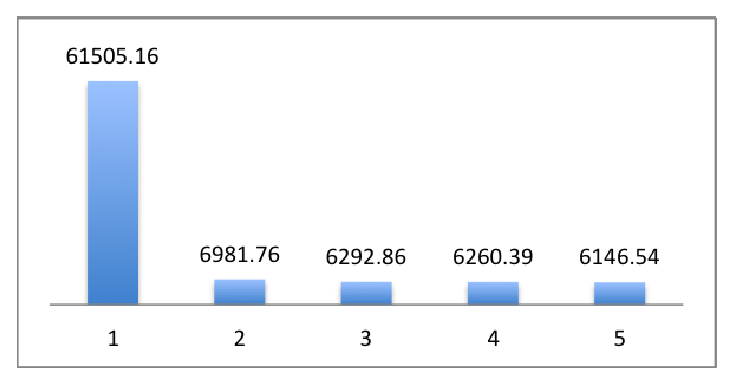
\includegraphics{perf_ngramlen1-5_itemsets_supp10+_1hr.eps}}
\rput(18.89,0.5441601){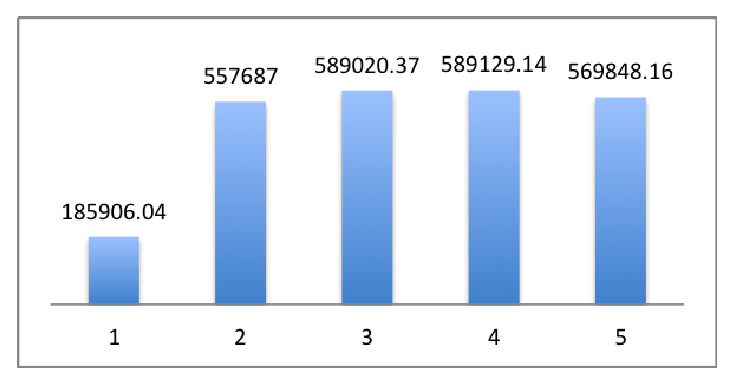
\includegraphics{perf_ngramlen1-5_distinct-items_supp10+_1hr.eps}}
\rput(31.89,0.50416017){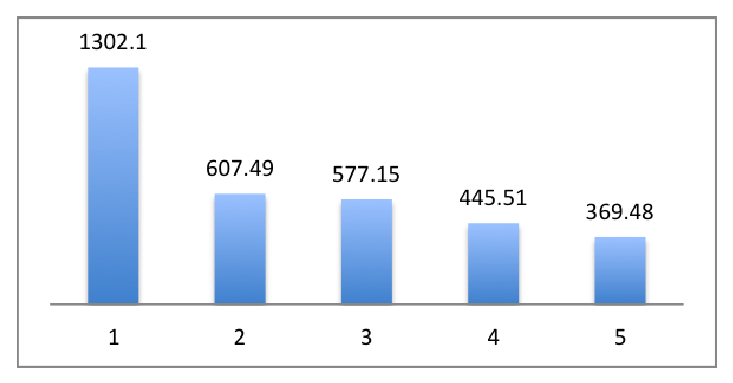
\includegraphics{perf_ngramlen1-5_runtime-millis_supp10+_1hr.eps}}
\end{pspicture} 
}
\caption{Effect of the increasing maximum N-Gram length on results of mining of 1hr epochs of data}
\label{fig:ngramsLen}
\end{figure*}


A large number of itemsets are language constructs that bear no information,
such as ``such as''. 
By treating sequential language constructs, and any other multiword expression,
as one item we eliminate a large number of such itemsets.
We can also eliminate itemsets that are made up of all the different fragments
of the language construct along with other items;
for example, \{we, did, it, \#teamobama\} can produce 10 other combinations of
length 2 or more.
There are many measures of association that can be used to detect multiword
expressions, but each measure is good only under certain conditions~\cite{ramisch2012broad,tan2002selecting}.
After preliminary experiments with various measures, we determined that
the best performance
could be obtained by tokenizing the documents into term N-grams with varying N. 

We use term N-gram tokens such that N-grams of high probability are replaced by
(N+1)-grams, resulting in a distribution with no high peaks.  
An N-gram is considered to 
have a high probability if its maximum likelihood estimate from a background
model is higher than a threshold $\eta_N$. 
A background language model built from a long epoch of data 
from the same stream is used for probability estimation.
The tokenization of a tweet starts by tokenizing it into unigrams, then each
unigram of high probability is replaced by two term bigrams~--~by
attaching to it the unigrams before and after it.
We keep replacing N-grams of high probability by two (N+1)-grams 
until there are no more such N-grams. 


The threshold of high probability, $\eta$, is different for each value of N. 
The threshold for unigrams is determined as follows: 
We pick a topical term that is known to  steadily  appear with a rather high frequency, 
and is talked about in all languages; for example, `obama'. 
The maximum likelihood estimate of the probability of the term `obama' 
is P(``obama") = 0.0001, which we use as $\eta_1$.
At each N, the probability threshold is adjusted to account for the increase
in the number of tokens and the overall increase in the grand sum of counts (caused by overlap).
The adjusted $\eta_N$ is:
\begin{equation}\eta_N = \eta_1 \times \frac{\sum_{\{w:\, w \,\in\, W\, and\, w.length \,\le\, N\}}{freq(w)}}{\sum_{\{v:\, v\, \in\, W \,and \,v.length\,=\,1\}}{freq(v)}}\end{equation}


Figure \ref{fig:ngramsLen} shows the effect of increasing the maximum length
of N-grams from 1 to 5 on 
the number of closed itemsets,
the number of tokens, 
and the runtime of mining one hour of data.
The values shown are averages across all one-hour epochs in the month of
November 2012.
Figure \ref{fig:ngramsLen}(a) shows that the number of itemsets 
drops by about 90\% by using variable length N-grams,
which overcomes the problem of mining language constructs
while limiting the increase in the sparsity of the data.
Figure \ref{fig:ngramsLen}(b) shows that the number of distinct items
increases substantially as N goes from 1 to 2, then continues increasing
slightly until it starts decreasing at N $\le$ 5. %N=5.
The decrease happens because 
some tweets are tokenized into less 5-grams than 4-grams,
eliminating 4-grams not appearing elsewhere.
Figure \ref{fig:ngramsLen}(c) shows that runtime also decreases as N goes
from 1 to 5, since the runtime of LCM  is proportional to the number of closed
itemsets, %CAN DELETE THE FOLLOWING LINE 
and is not affected by the increasing sparsity of data.


%\section{Filtering itemsets}
\section{Selecting Itemsets} 
\label{sec:strong}



In the previous section, we discussed our handling of function words,
using a technique that exploits LCM's tolerance to sparsity.
After applying this technique, the average number of itemsets mined from an
hour of twitter data drops from 61,505 to 6,146.
However, there is still redundancy in the itemsets.
For example, figure \ref{fig:sham} illustrates  itemsets related to Donald
Trump's famous tweets in reaction to Obama's victory in
2012\footnote{\scriptsize \url{http://www.huffingtonpost.com/2012/11/07/donald-trump-election-revolution_n_2085864.html}}.  
Each area in the figure represents the transactions containing the itemset
formed by concatenating the items in all intersecting ellipses. 

The closed property of an itemset is easily satisfied by an itemset
created through the modification of 
transactions that contain another closed itemset.
For example, if a transaction containing a closed itemset
is modified by removing one of its items,
another closed itemset with enough support is immediately formed.
While an update operation is not supported in the model of frequent itemset mining, 
a similar effect happens when people retweet, 
or even when they are writing original posts about 
a certain fine grained topic.
In case of retweeting, people actually start from the original tweet and 
then remove parts of it,
to make space for their content
or to keep only the part they want to emphasize. 
For example, in figure~\ref{fig:sham}  the most discriminative words are ``sham, and, travesty''
which are quoted 
%along with Donald Trump's user name 
in most of the retweets.
We can imagine that for each fine grained topic there is also a base post
that represent the information or ideas within the topic. 
People make posts about the fine grained topic 
by selecting parts of the base post
and adding their own thoughts.
This results in many closed itemsets 
about the topic that
are trivially different from each other.

The fact that any \emph{maximal} itemset is a closed itemset
is another \emph{weakness}. % of the closed condition.
If a closed itemset is expanded by certain items a number of times
over the support threshold, this results in a maximal itemset
which is closed by definition.
Now consider a tweet that is retweeted hundreds of times, 
and a small group of people appends the same words to it.
Since  a low support threshold has to be used when mining text,
this will result in a maximal itemset that
might not be adding any information to the closed itemset.
For example, in figure~\ref{fig:sham} a number of people
talked about ``hair'' along with ``sham, and, travesty''. 
The number is higher than the support threshold,
but it is relatively small within the topic.
%While amusing, this addition is not important.

We propose two conditions that are not as easily satisfied as the closed
condition for selecting itemsets.
The two conditions build on the concept of \emph{association rule confidence}.
Mining itemsets based on the confidence of rules they induce has long been
recognized as a method for finding
``interesting patterns'' \cite{cohen2001finding},
but since this property is not anti-monotone 
it cannot be directly used.
The confidence of an association rule that the presence of an itemset,
$s_{anteced.}$, implies the presence of another itemset, $s_{conseq.}$, is  defined as:
\begin{equation}\label{eq:conf}conf(s_{anteced.} \rightarrow s_{conseq.}) = \frac{|T_{s_{conseq.}} \cap T_{s_{anteced.}}|}{|T_{s_{anteced.}}|}\end{equation}



\begin{figure}
\centering
\resizebox{7cm}{3.5cm}
{
\begin{pspicture}(0,-2.649212)(9.077745,2.95)
\psframe[linewidth=0.04,dimen=outer](8.843161,2.95)(0.2431605,-2.61)
\usefont{T1}{ptm}{m}{n}
\rput(4.103317,1.675){sham, and, travesty}
\usefont{T1}{ptm}{m}{n}
\rput(1.7484828,2.575){@realdonaldtrump}
\pscircle[linewidth=0.04,dimen=outer](4.1031604,0.01){2.28}
\rput{55.644855}(2.9522903,-5.6005197){\psellipse[linewidth=0.04,dimen=outer](6.782275,-0.0031560312)(1.9103949,2.0626228)}
\rput{34.21703}(0.13301769,-1.7201583){\psellipse[linewidth=0.04,dimen=outer](2.8607624,-0.6440031)(2.908739,0.81)}
\pscircle[linewidth=0.04,dimen=outer](4.5031605,-0.33){1.58}
\usefont{T1}{ptm}{m}{n}
\rput(4.527965,-0.865){not,}
\pscircle[linewidth=0.04,linestyle=dashed,dash=0.16cm 0.16cm,dimen=outer](2.6031604,0.81){0.48}
\usefont{T1}{ptm}{m}{n}
\rput(1.0566566,1.455){fraud}
\pscircle[linewidth=0.04,linestyle=dashed,dash=0.16cm 0.16cm,dimen=outer](1.0631605,1.45){0.46}
\usefont{T1}{ptm}{m}{n}
\rput(2.623102,0.815){hair}
\pscircle[linewidth=0.04,dimen=outer](7.3231606,-1.35){1.02}
\usefont{T1}{ptm}{m}{n}
\rput(7.337262,-1.025){the, world, }
\usefont{T1}{ptm}{m}{n}
\rput(7.264635,-1.325){is, laughing}
\rput{34.21703}(0.8391447,-4.3701773){\psellipse[linewidth=0.04,dimen=outer](7.5185595,-0.8219682)(1.3607179,0.95923364)}
\rput{34.21703}(0.3818179,-4.274056){\psellipse[linewidth=0.04,dimen=outer](7.133755,-1.5167968)(1.2777647,0.86427283)}
\usefont{T1}{ptm}{m}{n}
\rput(7.207018,-1.645){at}
\usefont{T1}{ptm}{m}{n}
\rput(8.076705,-0.165){us}
\usefont{T1}{ptm}{m}{n}
\rput(6.371842,-2.105){you}
\usefont{T1}{ptm}{m}{n}
\rput(1.4102015,-1.625){elections}
\usefont{T1}{ptm}{m}{n}
\rput(6.9122915,1.255){rt}
\usefont{T1}{ptm}{m}{n}
\rput(4.4461293,-1.265){democracy}
\end{pspicture} 
}

\caption{Closed, distinct and strongly closed sets}
\label{fig:sham}
\end{figure}


\subsection{Distinct Itemsets}


The \emph{distinct} condition is a novel strengthening of the closed condition
so that it is not as easily satisfied. 
We define a \emph{distinct} itemset as a closed itemset whose frequency
comprises more than a certain proportion of the frequency of its least
frequent subset~--~we call this its \emph{parent} itemset. 
The proportion is a parameter, $\kappa$, that controls the selectivity of the
\emph{distinctiveness} condition.
This can be interpreted as selecting itemsets which are implied by a subset
with confidence greater than $\kappa$.
Formally, the set of \emph{distinct} itemsets, $\mathcal{D}$,
is defined as follows:
\begin{equation}\mathcal{D} = \{s: s \in \mathcal{C} \, and \, \exists \; s_{parent} \subset s \; where \; \frac{|T_{s}|}{|T_{s_{parent}}|} \ge \kappa 
\}
\end{equation}


In figure \ref{fig:sham}, \emph{distinct} itemsets are illustrated in solid
lines, and closed itemsets that do not satisfy the distinctiveness condition in dashed lines.
It is clear from the figure that considerable redundancy remains in
\emph{distinct} itemsets.

\subsection{Strongly Closed Itemsets}
To overcome the redundancy in \emph{distinct} itemsets 
we merge similar ones
into \emph{strongly closed} itemset clusters.
This will also filter out any itemset 
that does not belong to a particular topic
since it will not be part of a cluster.
The similarity of a \emph{distinct} itemset,
$s_d$, and another distinct itemset, $s_c$,
is measured as the overlap of the \emph{transactions} containing both of them
with the transactions containing $s_c$. 
A \emph{distinct} itemset is clustered with another itemset if one exists
such that the overlap exceeds a similarity threshold,
which we take to be $1-\kappa$ (the indistinctiveness of $s_d$ from $s_c$).
If more than one satisfies this condition,
the  \emph{distinct} itemset is clustered with the 
one having the highest overlap ratio.
When  a \emph{distinct} itemset is clustered with an itemset that is already
part of a cluster, the \emph{distinct} itemset is added to the existing cluster.
Finally, the \emph{strongly closed} itemset is the union of all cluster members,
and its postings lists is the union of their postings lists.
We define the  desired clustering  and the strongly closed itemset
represented by each cluster as follows:
\begin{align*}\label{eq:strongClosedFormal}
\mathcal{R} = \{r: r = \bigcup_i{(s_i, s_j)}\; where\; s_i \in \mathcal{D} \, and \, s_j \in \mathcal{D} 
\\\,and\; \forall_{(s_i,s_j)} \, s_j = \textbf{argmax}_{s_k} conf(s_k \rightarrow s_i) \\\,and \;conf(s_j \rightarrow s_i) \ge (1-\kappa)
\\\, and\;( s_j = r.centroid\; or \; (s_j, r.centroid) \in r )\}
\end{align*}
\begin{equation}S_l = \{w:\, w \in \bigcup_{(s_i, s_j) \in r_l}{s_i} \; where \; r_l \in \mathcal{R}\}\end{equation}

Confidence is not a symmetric measure,
but our proposed clustering makes use of the order
in which PPC-Extension generates itemsets 
to determine which itemset should be the antecedent 
and which should be the consequent.
If PPC-Extension uses a total ordering 
of items that is non-increasing in item frequency,
then 
an itemset generated earlier 
should be the antecedent, and
an itemset generated later
should be the consequent.
This builds upon the use of
variable length N-grams
as items,
so that the most frequent items
are not function words.
In that case, following the non-increasing order 
of item frequency leads to mining itemsets related 
to a certain topic close to each other.
Notice that PPC-Extension is equivalent to a depth first traversal 
of a hypothetical prefix tree of closed itemsets.
That is, closed supersets of each itemset are generated before 
moving to an itemset that is not a superset. 

The most discriminative itemset from each topic 
is mined before other itemsets from the same topic.
If an itemset branches out into supersets related to two topics 
or two opinions within one topic, this itemset is 
mined before itemsets from 
either of the two branches. It should not 
be clustered with either of the branches.
For an itemset to belong to a topic, it must contain a set of topical words. 
Since we are processing items in descending order of frequency, 
then itemsets containing multiple topical words are generated
when mining the supersets of the itemset containing only 
the most frequent of them.
According to these observations, 
the \emph{topical} similarity between itemsets
can be indicated by
the confidence of 
the association rule that
an itemset generated earlier implies 
an itemset generated later.

This clustering can be implemented efficiently using techniques similar to
the ones proposed by Bayardo et al. \cite{bayardo2007scaling}.
The main ideas are to limit the comparisons to a few candidates,
and to terminate the comparison early if the similarity threshold will not
be met.
In our case, the postings lists are longer than the itemsets,
so we generate candidates for comparison by calculating similarity between
itemsets.
When calculating the similarity between two postings lists,
we can terminate early if the difference exceeds the maximum difference
permissible to achieve a similarity of $1-\kappa$,
which can be derived from equation \ref{eq:conf}. 

Algorithm~\ref{algo:alliance}  shows a possible implementation.
For each itemset, $s_i$, we find the itemsets produced before it
and overlapping with it in one or more items.
Then we find the candidate, $s_c$, that maximizes
$conf(s_c \rightarrow s_i)$ such that the confidence exceeds $1-\kappa$.
Notice that confidence is not a symmetric measure,
and we only check the confidence of the rule that the clustering candidate
implies the itemset. 


\begin{algorithm}[t]
\SetAlgoLined
\LinesNumbered
\KwIn{$\kappa$: Minimum distinctiveness threshold} 
\KwData{$\mathcal{C}$: Closed itemsets produced by LCM}
\KwResult{$\mathcal{R}$: Strong closed itemset clusters}
\For{$i \gets 2$ to $|\mathcal{C}|$}{
	$C \gets \{s_c: s_c \in \mathcal{C} \, and \, c < i \, and \, |s_c \cap s_i| > 0\}$\;
	$P \gets \{s_p: s_p \in \mathcal{C} \, and \, p < i \, and \, s_p \cap s_i = s_p\}$\;
	$s_p \gets \textbf{argmax}_{s_p \in P}\frac{|T_{s_i}|}{|T_{s_p}|}$ \tcp*{Direct parent}
	\uIf{$s_p = null$ \textbf{OR} $\frac{|T_{s_i}|}{|T_{s_p}|} < \kappa$}{continue\tcp*{Not a distinct itemset}}
	$s_m \gets null$, $maxConf \gets 0$ \tcp*{Best clustering}
	\ForEach{$s_c \in C$}{
		$\Delta \gets (1 - (1-\kappa)) |T_{s_c}|$ \tcp*{Maximum difference}
		$\delta \gets$ difference($T_{s_c},T_{s_c \cup s_i},\Delta$) \tcp*{Stops early}
		
		\If( \tcp*[f]{Confidence $\ge$ threshold}){$\delta \le \Delta$}{ 
			$conf \gets \frac{|T_{s_c}| - \delta}{ |T_{s_c}|}$\;
			\If{$conf > maxConf$}{
				$s_m \gets s_k$ \tcp*{Best merge candidate}
				$maxConf \gets conf$ \;
			}
		}
	}
	\If{$s_m \ne null$}{
		\lIf(\tcp*[f]{New cluster}){$\mathcal{R}[s_m] = null$}{$\mathcal{R}[s_m] \gets s_m$} 
		$\mathcal{R}[s_i] \gets \mathcal{R}[s_m]$ \tcp*{Add $s_i$ to the cluster}
		$\mathcal{R}[s_m].itemset \gets \mathcal{R}[s_m].itemset \cup s_i \cup s_m$\;
		$\mathcal{R}[s_m].postingsList \gets \mathcal{R}[s_m].postingsList \cup s_i.postingsList \cup s_m.postingsList$\;
	}}
\Return{$\mathcal{R}$}\;
\caption{Forming strongly closed itemset clusters}
\label{algo:alliance}
\end{algorithm}



\subsection{Performance Analysis}
\label{sec:bounding}



Unlike the original LCM algorithm, filtering low confidence itemsets requires
us to keep mined results in memory to calculate the confidence of newly
generated ones.
The memory requirement is not large because the number of itemsets 
averages at about 6,000.
In our experience with the Twitter data, it was enough to keep only a buffer
of 1,000 itemsets when mining an hour long epoch.
This is based on the observation that the number of positions 
between an itemset and a clustering candidate 
is 1,973.11 on average, with a standard deviation of 1,443.64. 
The large standard deviation indicates that
candidates are either found close to the itemset
(less than 500 positions behind),
or in a position that is several thousands 
of itemsets behind. 
%Thus we keep only 1,000 itemsets.

Following is an analysis of
the performance of the filtering conditions proposed,
in terms of the number of itemsets after their application,
and the runtime overhead they add on top of 
the runtime of the LCM algorithm.
The experiments were run using a single threaded Java implementation of
algorithm \ref{algo:alliance},
running on a 1.4GHz processor with 2MB of cache.
We apply the algorithm to the mining results of all 
one-hour long epochs in the Twitter data.
Before filtering, the average number of itemsets mined 
from an hour-long epoch is
2,439.17 closed itemsets of length 2 or more;
that is, excluding itemsets that are merely a frequent item. 


Figure \ref{fig:kappa} show the effect of varying $\kappa$ on the mean number
of \emph{distinct} and \emph{strongly closed} itemsets.
The number of \emph{distinct} itemsets drops as the distinctiveness threshold
increases.
On the other hand, the number of \emph{strongly closed} clusters %formed 
increases as the similarity (indistinctiveness) threshold decreases.
The dashed line shows that the number of unclustered distinct itemsets reaches
zero at $\kappa=0.5$, explaining why the number of clusters changes very
slightly after that. 
We use $\kappa = 0.25$ in the remainder of the paper,
which is an arbitrary choice based on the definition not the data.
The average size of an hourly synopsis
at this value of $\kappa$
averages at 139.1 \emph{strongly closed} itemsets.
%,
%and 85.38 \emph{distinct} itemsets. 


\begin{figure}
\scalebox{.5} 
{
\begin{pspicture}(0,-4.16)(16.6,4.16)
\rput(8.3,0.0){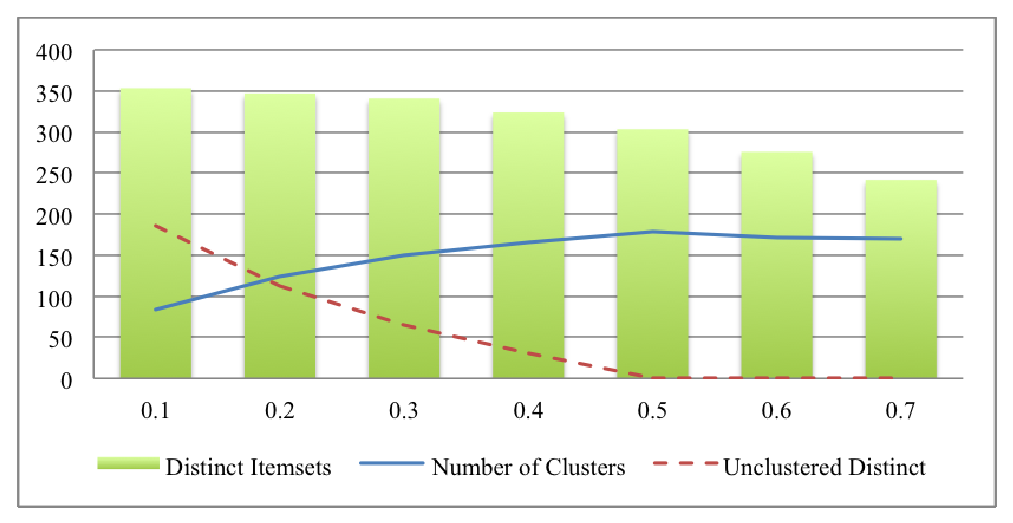
\includegraphics{kappa_effect.eps}}
\end{pspicture} 
}
\caption{Effect of changing $\kappa$ on mining results }
\label{fig:kappa}
\end{figure}



Figure \ref{fig:lcmvsfpzhu} shows the total runtime of the LCM algorithm plus
filtering based on the \emph{distinct} condition and clustering into \emph{strongly closed}
itemsets at different epoch spans.
The runtime of LCM alone is also plotted for reference.
We also plot the performance of another frequent itemset mining algorithm,
FP-Zhu \cite{grahne2004reducing}, which was the runner up at
FIMI 2004~\cite{DBLP:conf/fimi/2004}.
We include it to show that our extensions do not degrade the performance of
LCM even in the context of competitions.
The y-Axis is in logarithmic scale to keep the scale of the plot suitable for
seeing slight differences.
The output of LCM is the input to the filtering and clustering step,
so it is affected by the number of closed itemsets produced.
This explains why it takes slightly longer time for clustering results from
the 15-minute epoch and then takes 
a constant time for epochs of a longer span. 

These runtimes are achieved by using a buffer of 1,000 itemsets,
which is the same setting we use when evaluating the quality of the synopsis
in the next section.
If all itemsets are kept in memory the runtime increases slightly and
averages at 5.2 seconds for filtering a one-hour epoch.

\begin{figure}
\centering
\resizebox{9cm}{4.25cm}
{
\begin{pspicture}(0,-4.52)(16.408476,4.52)
\rput(7.52,0.0){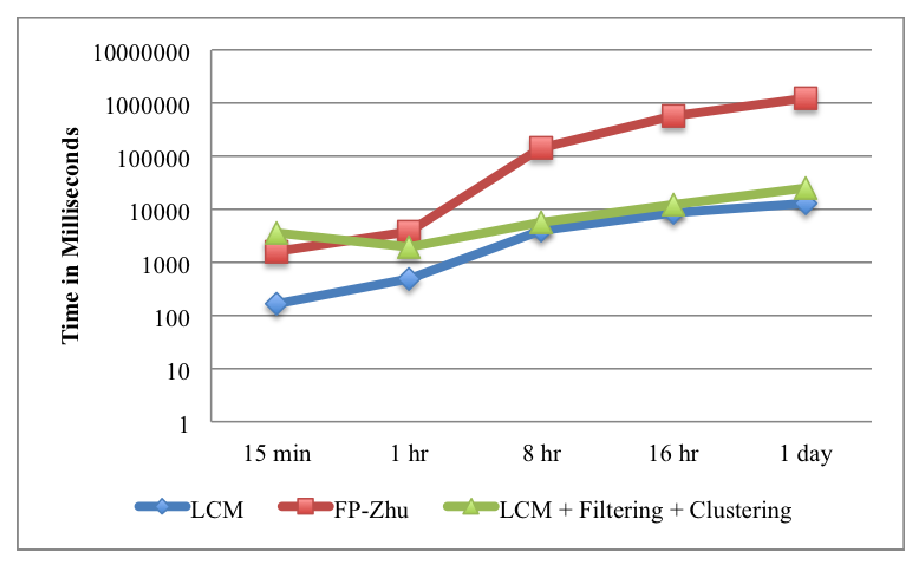
\includegraphics{runtime_lcm-lcm+filter-fpzhu_seconds.eps}}
\usefont{T1}{ptm}{m}{n}
\rput(14.1,-3.85){\large ($\kappa = 0.25$)}
\end{pspicture} 
}
\caption{Runtime of itemset mining alone and with filtering and clustering at different epoch spans}
\label{fig:lcmvsfpzhu}
\end{figure}

\section{Temporal Ranking}
\label{sec:rank}
The previous filtering steps reduce the number of itemsets to 
under 10\% of their original number.
In this section, we present a method for ranking itemset clusters 
such that they can
be presented to users in rank order
as a summary of events in the epoch.
The ranking can also be
used as input to additional search or
summarization steps.

We rank \emph{strongly closed} itemsets according 
to their temporal novelty,
compared to 
a longer period of time 
leading up to the mined epoch
--~a background model.
A good indicator of novelty is the point-wise Kullback-Leibler Divergence (KLD)
between an itemset's probability in the current epoch and in the background model.
The KLD of the probability of an itemset, $s_i$, in the background
model, $Q$, from the current epoch's model, $P$, can be considered as
the Information Gain, IG, in moving from a prior to a posterior distrubtion: 
\begin{align}IG(P(s_i),Q(s_i))  &= - (H(P(s_i)) - H(P(s_i),Q(s_i))) \notag\\ &= \sum{P(s_i) \log{P(s_i)}} - \sum{P(s_i) \log{Q(s_i)}} \notag\\ &= KLD(P(s_i)||Q(s_i))\end{align}

To calculate the collective IG of a strongly closed itemset cluster,
we have to take into account that the itemsets of the cluster are not independent. 
For simplicity we will consider only the pairwise dependence between 
every itemset and the smallest common subset, $s_{min}$.
We also normalize by the size of the cluster, $m$, to avoid favouring large clusers. Hence, our ranking formula for
\emph{strongly closed} itemsets:
\begin{align}\label{eq:avgIG}score(r) &= IG(P(s_{min}), Q(s_{min})) \notag\\ &+ \frac{ \sum_{ j = i_1..i_m } { IG(P(s_j|s_{min}), Q(s_j|s_{min})) } } { m } \end{align}


\subsection{Empirical Evaluation}
\label{sec:empirical}
We now show examples of the synopses produced by ranking
the \emph{strongly closed} itemsets. 
The examples will serve as our assessment of the quality of 
the synopses. 
We make an effort to choose epochs from time periods when 
it is known what people should be talking about. 
We show how the 2012 U.S. presidential elections day is summarized by our methods. %hour-by-hour
We compare our summary to the one produced by a state of the art algorithm, MTV,
which generates better quality summaries than other summarization algorithms based on itemsets~\cite{mampaey2011tell}. 
We also investigate the synopses of hours selected by the aid of Google Trends,
%\footnote{\scriptsize \url{http://www.google.ca/trends}},
assessing which popular queries were or were not reflected in our synopses.

\subsubsection{U.S. Presidential Elections Day}
Table \ref{table:nov6} shows the top 3 \emph{strongly closed} itemsets
from one-hour epochs on the elections day.
The itemsets shown are the first appearances of the most interesting itemsets;
that is, an hour is shown only if its top 3 feature novel interesting itemsets.
The first column is the beginning of the hour, EST time.
The second column is the top itemsets, 
reordered and punctuated to be meaningful phrases 
by looking at a few tweets from the postings list of each itemset.
The third column is a commentary to explain the itemsets,
also composed according to tweets in the postings lists.
The fourth column is the rank of an equivalent itemset 
in the top 30 itemsets mined by the MTV algorithm, if one exists.

Table~\ref{table:mtv} shows the top 3 itemsets picked by MTV, 
for hours when they include interesting itemsets.
Each interesting itemset has
an equivalent \emph{strongly closed} itemset in the top 50 (actually less)\footnote{\scriptsize \url{http://
blinded.blinded.com/blinded/
%plg.uwaterloo.ca/~yaboulna/
thesis_results/twitter_synopses/elections-day_top50.txt}}.
%nov6-0500_nov7-0850_top50-strongly-closed.txt}}.
Its rank is in the second column.



\begin{table}
\begin{center}
\footnotesize
\def\arraystretch{1.2}
\begin{tabular}{|p{0.7cm}|p{2.5cm}|p{4cm}|c|}
\hline
\textbf{Time} & \textbf{Itemset} & \textbf{Explanation} & \textbf{M} \\ \hline
\multirow{3}{*}{\texttt{08:30}}
& \em get out and vote & Encouraging participation & 17 \\ \cline{2-4}
& \em \scriptsize happy elections day & Congratulations & 27 \\ \cline{2 - 4}
& \em it's elections day & Excitement  & - \\ \hline

\multirow{3}{*}{\texttt{09:30}}
& \em if romney wins & Reflecting about possiblities & - \\ \cline{2 - 4} 
& \em of your ballot & Telling people to stop sending pictures of their ballots & - \\ \cline{2-4}
& \em in line to vote & Tweeting while in line  & 28 \\ \hline

%\multirow{3}{*}{\texttt{15:00}}
%& \em Borusia Dortmnd Real Madrid 2 & Score of football match; no events related to elections & 17 \\ \cline{2 - 4}
%& \em incroyable talent & A TV show from France & - \\ \cline{2-4}
%& \em City Ajax 2 & Another football match & - \\ \hline

\multirow{3}{*}{\texttt{19:30}}
& \em Linda  McMahon		&  She loses CT senate race & - \\ \cline{2 - 4}
& \em Florida is so ... & tight or close; the vote count  & - \\ \cline{2-4}
& \em \small Romney is winning & Speculations about results  & - \\ \hline 


\multirow{3}{*}{\texttt{20:00}}
& \em New Hampshire &  Obama won in NH & 9 \\ \cline{2 - 4}
& \em Obama to win / is winning & Two itemsets speculating  & - \\ \cline{2-4}
& \em too close to call & The results are still not clear & 22 \\ \hline


\multirow{3}{*}{\texttt{21:00}}
& \em Ohio and Florida &  Obama won in 2 more states & - \\ \cline{2 - 4}
& \em Sarah Palin & Sarah Palin  on Fox news  & - \\ \cline{2-4} 
& \em concession speech & Todd Akin's  speech & - \\ \hline


\multirow{5}{*}{\texttt{22:00}} 
& \em The electoral college &  Republicans complaining about the voting system  & 9 \\ \cline{2 - 4}
& \em President of the United States & Barack Obama is the 44th president of the USA   & 8 \\ \cline{2-4} 
& \em who voted for & Taking things personally & - \\ \cline{2-4} 
& \em once you go black you never go & A popular culture reference, missing ``back''& 15 \\ 
%\cline{2-4} 
%& \em my president is black & Americans proud about the equality of opportunities & - \\
 \hline % 

\multirow{3}{*}{\texttt{22:30} }
& \em @realdonaldtrump this elections ... [complete tweet]	& Trump's ``sham and travesty'' tweets. This cluster merges 26 \emph{distinct} itemsets. & 1  \\ \cline{2-4}
& \em concede to & The loser has to concede  & - \\ \cline{2-4} 
& \em Obama won. I ... & Reactions to the result & - \\ \hline 

\multirow{3}{*}{\texttt{23:00} }
& \em same sex marriage	& Some states legalized same sex marriage & 27  \\ \cline{2-4}
& \em for recreational use & CO and WA legalized weed for recreational use   & 21 \\ \cline{2-4} 
& \em acceptance speech & Anticipation for the speech & 26 \\ \hline 

\multirow{3}{*}{\texttt{00:30} }
& \em Delivered, sealed, signed & Stevie Wonder's song used in Obama's campaigns & 10  \\ \cline{2-4}
& \em The best is yet to come & Quote from Obama's acceptance speech  & 2 \\ \cline{2-4} 
& \em with the flag in her [hair]	&  During the speech, attention goes to a woman appearing behind Obama on TV! & 14 \\ \hline 
						
\end{tabular}
\end{center}
\vspace{-5mm}
\caption{Top 3 \emph{strongly closed} itemsets for hours in US presidential elections day (November 6, 2012)} 
 \label{table:nov6}
\end{table}

 \begin{table}
 \begin{center}
\small
\def\arraystretch{1.2}
\begin{tabular}{|p{7.5cm}|c|}

\hline
\textbf{Itemset} (with [tweet id] if the itemset is a whole tweet) & \textbf{S} \\ \hline

@realdonaldtrump,this,elections,...[266035509162303492] & 1
\\ \hline
 %This election is a total sham and a travesty. We are not a democracy! 
we, re, all, in, this, together, ..., bo [266031109979131904]  & 22 \\ \hline
 % That's how we campaigned, and that's who we are. Thank you. -bo
@realdonaldtrump,our,country,is,...[266037143628038144]  & 24 \\ \hline
%Our country is now in serious and unprecedented trouble...like never before.
\specialrule{.1em}{.05em}{.05em} 


URL,and,autotweet,checked,followed,me,today,unfollowed & N/A \\ \hline

house,of,representatives,shouldnt,...[266040877552656385] & 15 \\ \hline
% House of Representatives shouldn't give anything to Obama unless he terminates Obamacare.
 URL,\#android,\#androidgames,\#gameinsight & N/A \\ \hline
\specialrule{.1em}{.05em}{.05em} 

URL,and,autotweet,checked,followed,me,today,unfollowed & N/A \\ \hline
URL,\#android,\#androidgames,\#gameinsight  & N/A \\ \hline
@barackobama,@ryanseacrest, what, was, your, first, words, in, reaction, to, re, election, 2 & 36 \\ \hline 
\specialrule{.1em}{.05em}{.05em} 
URL,and,autotweet,checked,followed,me,today,unfollowed & N/A \\ \hline
the, best, is, yet, to, come & 2 \\ \hline
 URL,\#android,\#androidgames,\#gameinsight & N/A \\ \hline
 

\end{tabular}
\end{center}
\caption{Top 3 picked by the MTV algorithm}
 \label{table:mtv}
\end{table}

\subsubsection{Google Trends}
We use the Top Charts of November 2012 
for the people category\footnote{\scriptsize 
\texttt{http://www.google.ca/trends/explore\#q=Justin\%20Bieber\%2C\%20\\
Taylor\%20Swift\%2C\%20Rihanna\%2C\%20Nicki\%20Minaj\%2C\%20\\
Selena\%20Gomez\&geo=US\&date=11\%2F2012\%201m\&cmpt=q}}
as an aid for finding out what social media users
are expected to be talking about.
We observed that named entities that make it to the top 10 chart in the people 
category  are divided into finer groups. 
The queries about 
people in each group 
have similar volumes over time, 
with peaks at the times of real world events
in which the people in the group took part.
Five out of the top 10 are pop artists, 
with high query volume at times of music awards events.

The top 30 \emph{strongly closed} itemsets mined from hours leading to 
the MTV Europe Music Awards contain
many itemsets about the events and the artists, 
especially that this event used social media to collect audience votes. 
Voting for the award winner is 
a good example of a topic where people have strongly different opinions.
Such different opinions are all reported as separate \emph{strongly closed} itemsets, 
because clustering in the transaction space avoids forming incohesive clusters. 
Moreover, different  \emph{strongly closed} itemsets from one such topic
can all occupy high ranks.
For example, the top 3 itemsets for 3 PM on November 9 are all variations of the 
itemset: \{i, think, ARTIST, NAME, will, be, the, big, winner, tweet, your, pick, at, URL, %\footnote{\scriptsize \url{http://ema-twittertracker.mtv.com/live/predict.html}}, 
\#mtvema\}; replacing ARTIST NAME by Justin Bieber, Katy Perry, or Lady Gaga and adding a hashtag for each artist.

One of the 5 artist does not appear in the itemset selection. 
The name of Rihanna never appeared in any \emph{strongly closed} itemset.
Actually it rarely appeared in any itemset of length 2 or more. 
This indicates that there was not enough support for any itemset
with her name (of length 1) and other information.
It is impossible for an itemset of length 1 to be selected,
since our proposed conditions select itemsets implied
by a subset with high confidence.
%Therefore \emph{distinct} and \emph{strongly closed} itemsets
%would never capture information in an itemset of length 1.


\section{Conclusion and future work}
\label{sec:concfut}
We have proposed adaptations for frequent itemset mining 
such that it can be efficiently and effectively applied to 
social media text.
We based our work on a frequent itemset mining algorithm that is suitable
for sparse data, LCM~\cite{uno2004lcm}.
The direct application of the LCM algorithm resulted 
in a large number of closed itemsets (on average 61,505.16 itemsets 
%for an hour of Twitter data)
per hour),
which are dominated by language constructs
and contain considerable redundancy and noise.
The result of the modified algorithm is a concise selection of
high quality itemsets (on average 139.1 itemsets 
per hour),
%for an hour of Twitter data),
which was shown to capture important events.
Moreover, the improvement in effectiveness does not tax
the efficiency of the algorithm.
Thus we provided a recipe for mining frequent itemsets
from social media text, starting from recommending
a suitable algorithm. Our main contributions are: 
(1) a novel method to avoid mining itemsets that are 
merely language constructs,
(2) a novel condition for selecting itemsets that are distinctively different, and
(3) an efficient clustering scheme to reduce redundancy.

We aim to exploit the synopses for temporal query expansion in our future work. Terms from itemsets relevant to a query (or occurring in a relevant document)
can be used for query expansion, thus acting as precomputed results of 
pseudo-revelance feedback.
We also wish to explore ways to make use of the temporal signal during mining,
such as when calculating similarity during clustering.

 

%\section{Acknowledgements}
% No Acknowledgments yet...
%This paper was funded in part by the Google Focus Award. Right?? What else should we say here? I am writing to fill some space and reserve it for the actual acknowledgements.
%% Thank YOU!


\small
% The following two commands are all you need in the
% initial runs of your .tex file to
% produce the bibliography for the citations in your paper.
\bibliographystyle{abbrv}
\bibliography{younos_wsdm2014}  % sigproc.bib is the name of the Bibliography in this case
% You must have a proper ".bib" file
%  and remember to run:
% latex bibtex latex latex
% to resolve all references
%
% ACM needs 'a single self-contained file'!
%
%APPENDICES are optional
%\balancecolumns

\end{document}
